\documentclass[11pt, a4paper]{article}
\usepackage{fullpage}
\usepackage[USenglish]{babel}
\usepackage{graphicx} 
\usepackage[small,bf,hang]{caption2}
\usepackage{nameref}
\usepackage{hyperref}
\hypersetup{
    colorlinks,
    citecolor=black,
    filecolor=black,
    linkcolor=black,
    urlcolor=black
}
\usepackage{pdfpages}
\usepackage[square]{natbib}


\title{Master Thesis -  Security Aspects in Virtual Networks\\ \textbf{SITREP 19}}
\author{\textbf{Laurent De Wilde} \\ Master of Science in the Applied Computer Science \\ Vrije Universiteit Brussel}
\date{May 18, 2015}

\begin{document}
\maketitle


\section*{Work done}
\begin{itemize}
\item Installed the Juniper vSRX security appliance in my network. However, the download came as a VMWare appliance, so I first had to convert the .vmdk file to a .vhd file in order to run it on Hyper-V. However, the Hyper-V is not supported by the vSRX. I tried to install it in Hyper-V and Xen, but the network cards were not identified. I tried various settings and workarounds, such as ``Hyper-V Integration Services'' and different kinds of network modes, but neither of them worked. \\
So that is why I installed the vSRX appliance in VirtualBox. This approach worked for me.
\item Performed the first configuration steps. The vSRX comes as a lockdown device, so first I had to enable ICMP, HTTP and SSH access. Therefore, the cli and configuration mode had to be started with the commands \texttt{cli} and \texttt{configure} respectively. \\
Then, the initial setup of the device:
\begin{itemize}
\item \textbf{Set the host name:} \texttt{set system host-name}
\item \textbf{Set root password:} \texttt{set system root-authentication plain-text-password}
\item \textbf{Show the interfaces to set up static IP:} \texttt{show interfaces terse}
\end{itemize}
$\;$ \\ \\
\noindent\begin{minipage}{\textwidth}
    \centering
    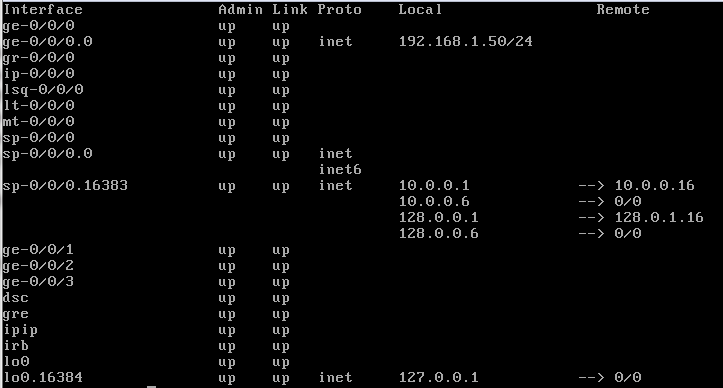
\includegraphics[width=\textwidth]{Juniper_2.png}
 \captionof{figure}{The interfaces list}
\end{minipage}
\begin{itemize}
\item \textbf{Set static IP:} \texttt{set intefaces ge-0/0/0.0 family inet address 192.168.1.50/24}
\item \textbf{Edit the security zone to allow certain traffic:} \texttt{set security zones security-zone untrust interfaces ge-0/0/0 host-inbound-traffic system-services ping ssh http}
\item \textbf{Save changes:} \texttt{commit}
\item \textbf{Exit:} \texttt{exit}
\end{itemize}
\end{itemize}
$\;$ \\ \\
A simple ping confirms the accessability of the device.
$\;$ \\ \\
\noindent\begin{minipage}{\textwidth}
    \centering
    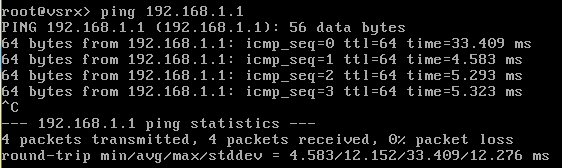
\includegraphics[width=\textwidth]{Juniper_3.png}
 \captionof{figure}{OK}
\end{minipage}
$\;$ \\ \\
With the initial configuration completed, the web interface can now be accessed:
$\;$ \\ \\
\noindent\begin{minipage}{\textwidth}
    \centering
    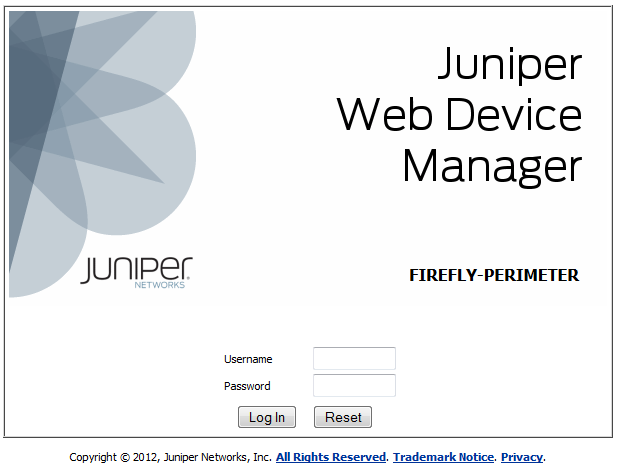
\includegraphics[width=\textwidth]{Juniper_1.png}
 \captionof{figure}{The home page.}
\end{minipage}

\subsection*{Penetration testing of vSRX}

Prior to investigating how the Juniper vSRX can protect a private cloud, the security of the device itself has been tested first. Therefore, some pentration testing using NMAP, Acuneticx web vulnerability scanner, 2 DOS tools and various tools available in Kali Linux. \\
The first step is the reconnaissance step: performing a system scan with NMap. \\
The \texttt{target} host is the Juniper vSRX appliance which has the IP address of 192.168.1.50. \\
The \texttt{command} executed is \texttt{nmap -T4 -A -v 192.168.1.50}, which scans the TCP ports 1-1024 for open ports, tries to detect the OS and the device type. It also tries to detect the version of the OS and performs a traceroute. This is an intrusive scan. \\
\paragraph{Results} As previously mentioned, the device comes as a lockdowned box, which means that all ports are closed. In the configuration process, some ports have been opened to allow web and SSH traffic. And indeed, the scan result shows that only ports 80 (HTTP) and 22 (SSH) are open. \\
The OS detection probe failed to correctly determine the running OS. It determined that the device is a mobile phone running Apple iOS. This has never happened before when using Nmap. This can be seen as positive behaviour: an intruder may think the device runs Apple iOS, while in fact it runs Juniper Junos version 12. This way, an intruder may try to exploit vulnerabilities specific to Apple iOS, but these will of course not work in this case. \\
The version of  the SSH server and webserver were correctly detected, being OpenSSH 6.6 and Embedthis-Appweb 3.2.3.
$\;$ \\ \\
\noindent\begin{minipage}{\textwidth}
    \centering
    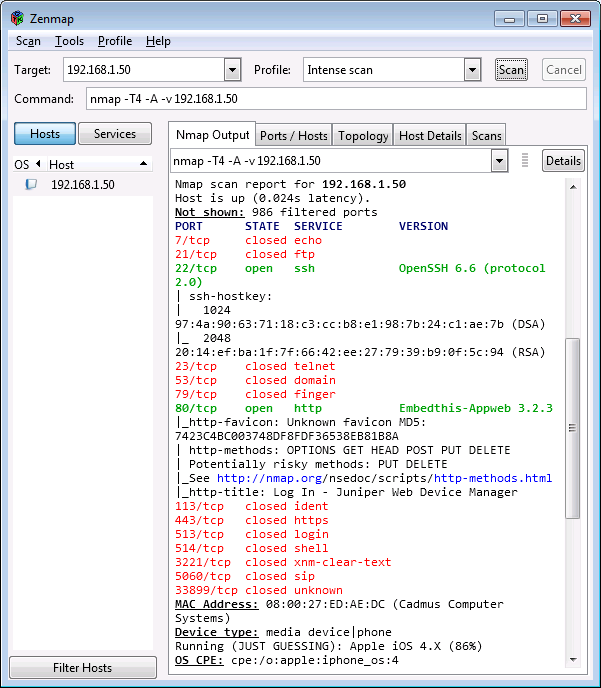
\includegraphics[width=\textwidth]{NMAP_1.png}
 \captionof{figure}{Nmap scan results}
\end{minipage}

\clearpage

In addition to the Nmap scan, the webserver has been tested for known exploits using Acunetix Web Vulnerability Scanner.
\paragraph{Results} First of all, a login sequence has been created, so the scanner has access to otherwise restricted pages. This way, the scanner can perform optimally. \\
The Acunetix Web Vulnerability Scanner classifies threat level of the website of vSRX as ``High''. The most important security issue is the Host header attack. \\
The host header is used to uniquely identify a web domain \citep{hostheader}. This is used because some servers host multiple websites on one server \citep{hostheader2}. However, the problem is that web applications insert this Host header value into their application code (the HTML page) without proper validation \citep{hostheader3}. This way, cache poisoning and password reset poisoning can be done.
\begin{itemize}
\item  Web Cache poisoning:  the Host header is replaced with a malicious hostname, or by using duplicate Host headers. This way, the cache is poisoned with URL's pointing to the malicious hostname \citep{hostheader3}. \\
Solution: don't use the Host Header value, but apply strict filters to only allow FQDN's.
\item Password reset poisoning: sometimes a website uses a link to reset a users's password. This link can contain the Host header provided by the person requesting the password reset. When replacing this Host header with a Hostname of the attacker, the link will link to the attacker's website.  Then, the attacker can retrieve the query string parameters \citep{hostheader3}
\end{itemize}
The affected items are: \texttt{/extjs/resources/themes/images/default/shared}, \texttt{/gui-framework/images} and \texttt{/images}.
$\;$ \\ \\
\noindent\begin{minipage}{\textwidth}
    \centering
    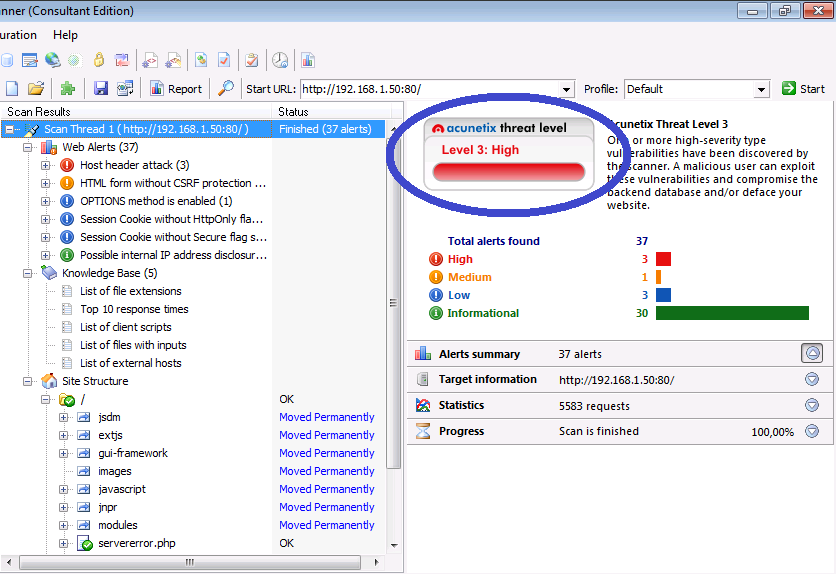
\includegraphics[width=\textwidth]{Acunetix_3.png}
 \captionof{figure}{Acunetix classifies the website's threat level as ``high'' .}
\end{minipage}
$\;$ \\ \\
\noindent\begin{minipage}{\textwidth}
    \centering
    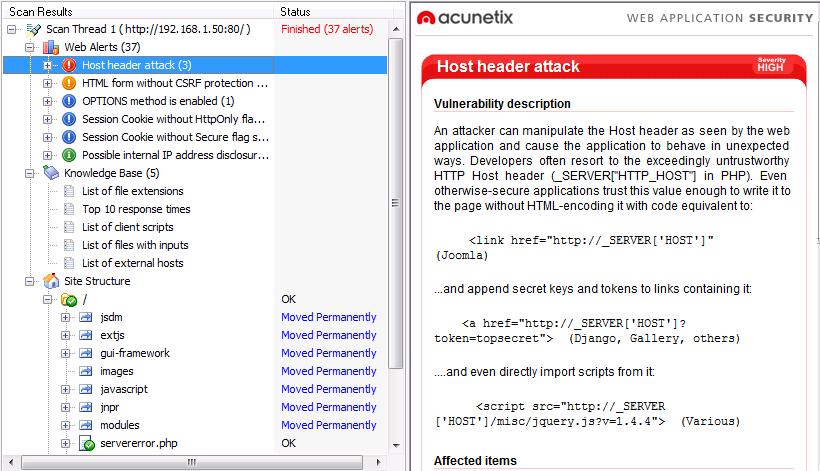
\includegraphics[width=\textwidth]{Acunetix_4.png}
 \captionof{figure}{Host header attack vulnerability.}
\end{minipage}
$\;$ \\ \\
Another (medium) threat found is ``HTML form without CSRF protection''. A Cross-Site Request Forgery is an attack where a website forces an authenticated user to execute an unwanted action, e.g.: making a payment or changing a password \citep{CSRF,CSRF2}. An attacker can use a HTML form that doesn't have CSRF protection to submit any information (or the information provided by the user that filled in the form) on the form to the attacker's website that displays a form similar as the original one. A solution could be to use a key, store it in the user's session and require it as an additional value if form submissions \citep{CSRF3}. \\
The affected item is the Login form at \texttt{/login}.
$\;$ \\ \\
\noindent\begin{minipage}{\textwidth}
    \centering
    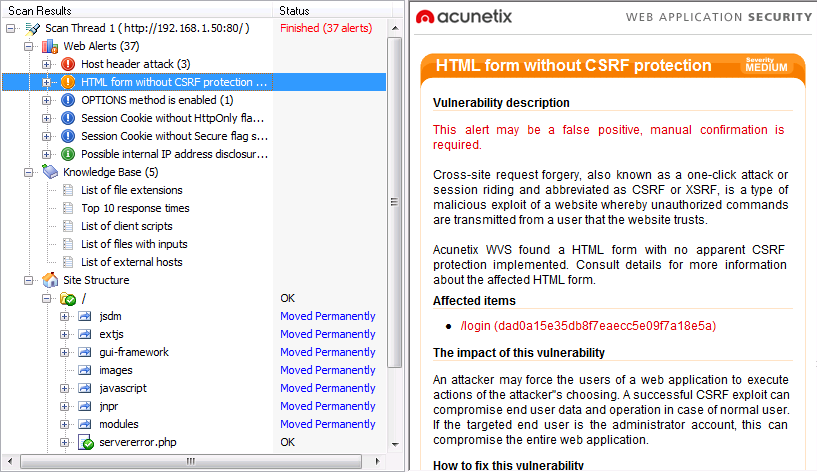
\includegraphics[width=\textwidth]{Acunetix_5.png}
 \captionof{figure}{Possible CSRF warning.}
\end{minipage}
$\;$ \\ \\
The next step is to try a DOS the security device. But first, I tried to use a sequence of login actions using Nessus to see how the device would response. While performing the operation, I was unable to open the site. I.e.: the browser kept showing a \texttt{Waiting for 192.168.1.50\ldots message}. When the operation has completed, I tried to open the website again. This worked, but when trying to login a message indicating that the maximum numbers of login sessions was reached was displayed.
$\;$ \\ \\
\noindent\begin{minipage}{\textwidth}
    \centering
    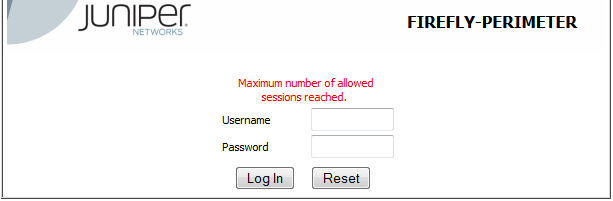
\includegraphics[width=\textwidth]{Juniper_4.png}
 \captionof{figure}{The maximum number of login sessions is reached.}
\end{minipage}
$\;$ \\ \\
Then three actual DOS attacks have been performed. One using the tool ``Hulk'', another one using the tool ``LOIC'' and yet another one using the tool ``DDOSIM''. \\
In all the cases, I was unable to reach the website as the tools were performing their attacks. However, when the attack was completed, only in the case of LOIC, the device remained unreachable and thus was successfully DOS'ed. \\
$\;$ \\ \\
\noindent\begin{minipage}{\textwidth}
    \centering
    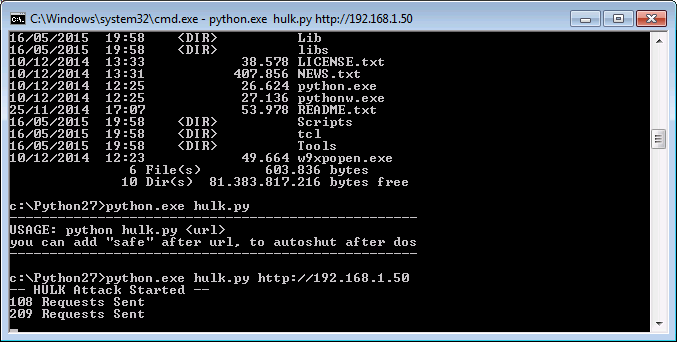
\includegraphics[width=\textwidth]{DOS_1.png}
 \captionof{figure}{Hulk in action\ldots .}
\end{minipage}
$\;$ \\ \\
\noindent\begin{minipage}{\textwidth}
    \centering
    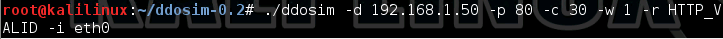
\includegraphics[width=\textwidth]{DDOSIM.png}
 \captionof{figure}{DDOSIM command.}
\end{minipage}
\clearpage
Then some more vulnerability scanning has been performed. This time, Nessus is used to perform advanced network scans and web application scans. \\
It turns out that Nessus detected quite a lot information in addition to Nmap. It detected the correct device type (embedded) and the correct OS (Juniper Junos). The version of the webserver was also successfully detected. The complete list is available in the Appendix.
$\;$ \\ \\
\noindent\begin{minipage}{\textwidth}
    \centering
    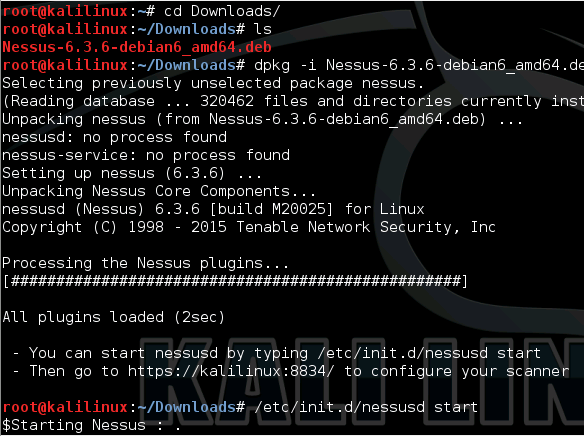
\includegraphics{Nessus_0.png}
 \captionof{figure}{Installation of Nessus on KaliLinux.}
\end{minipage}
$\;$ \\ \\
According to Nessus, three vulnerabilities have been found: \texttt{Web Server Uses Plain Text Authentication Forms}, \texttt{SSH Server CBC Mode Ciphers Enabled} and \texttt{SSH Weak MAC Algorithms Enabled}.
\noindent\begin{minipage}{\textwidth}
    \centering
    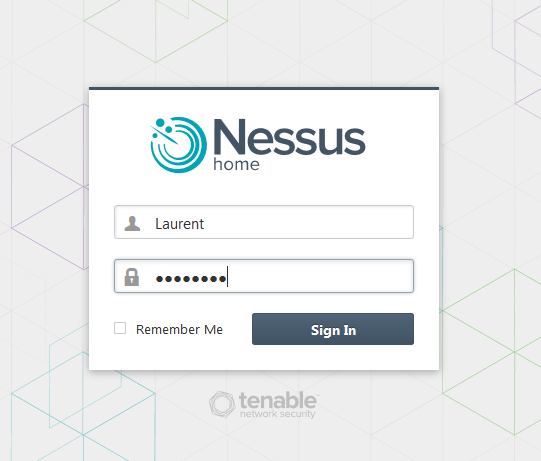
\includegraphics{Nessus_1.png}
 \captionof{figure}{The web interface.}
\end{minipage}
$\;$ \\ \\
\noindent\begin{minipage}{\textwidth}
    \centering
    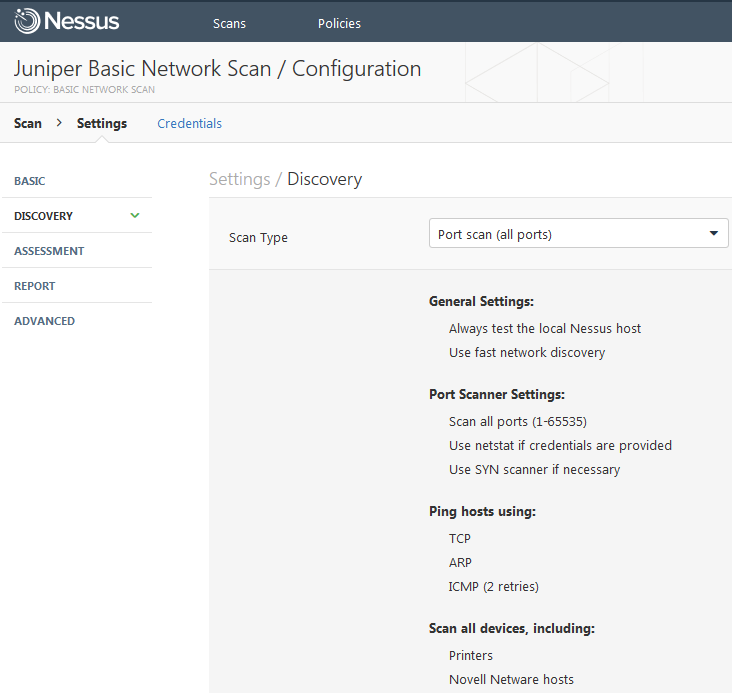
\includegraphics[width=\textwidth]{Nessus_2.png}
 \captionof{figure}{Basic scan settings.}
\end{minipage}
$\;$ \\ \\
\noindent\begin{minipage}{\textwidth}
    \centering
    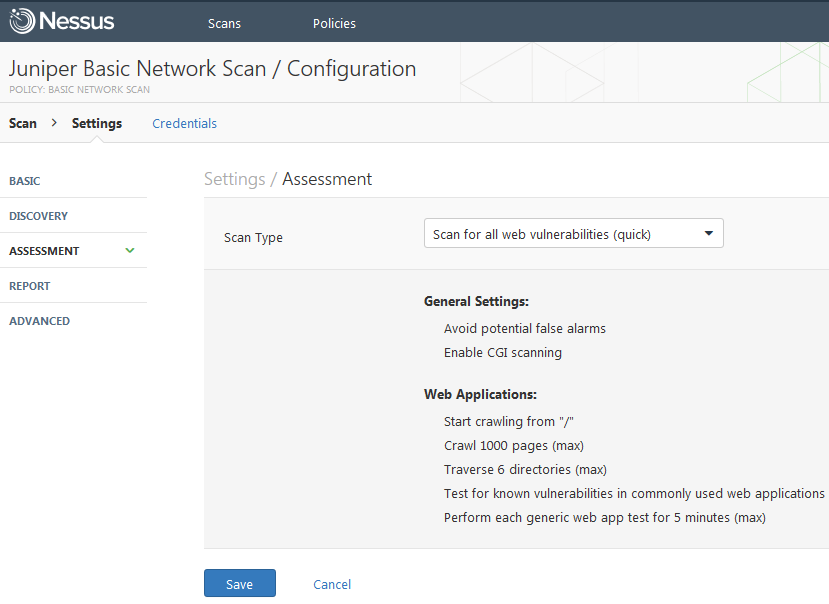
\includegraphics[width=\textwidth]{Nessus_3.png}
 \captionof{figure}{Basic scan settings.}
\end{minipage}
$\;$ \\ \\
\noindent\begin{minipage}{\textwidth}
    \centering
    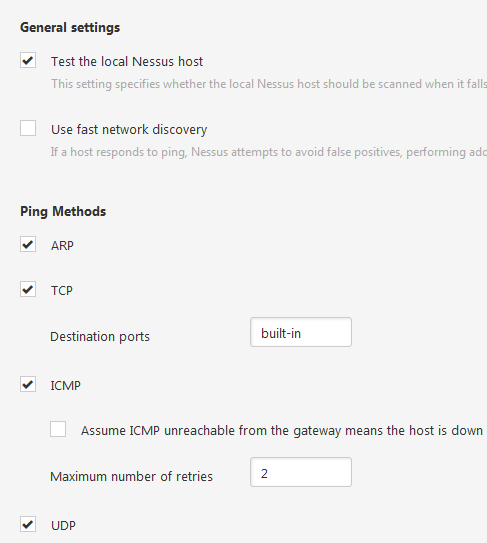
\includegraphics[width=\textwidth]{Nessus_5.png}
 \captionof{figure}{Advanced scan settings.}
\end{minipage}
$\;$ \\ \\
\noindent\begin{minipage}{\textwidth}
    \centering
    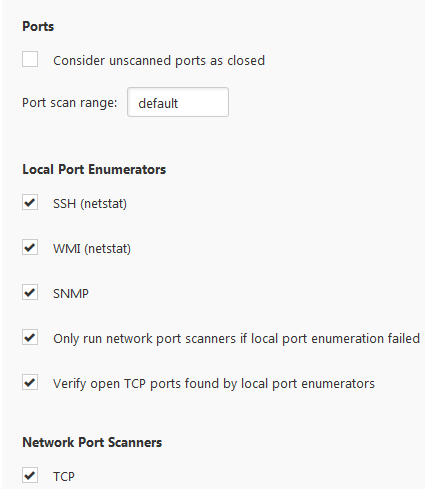
\includegraphics{Nessus_6.png}
 \captionof{figure}{Advanced scan settings.}
\end{minipage}
$\;$ \\ \\
\noindent\begin{minipage}{\textwidth}
    \centering
    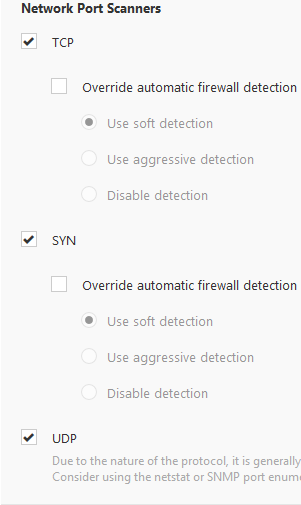
\includegraphics{Nessus_7.png}
 \captionof{figure}{Advanced scan settings.}
\end{minipage}
$\;$ \\ \\
\noindent\begin{minipage}{\textwidth}
    \centering
    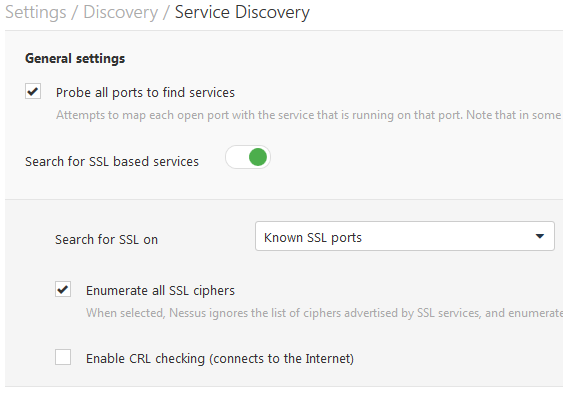
\includegraphics[width=\textwidth]{Nessus_8.png}
 \captionof{figure}{Advanced scan settings.}
\end{minipage}
$\;$ \\ \\
\noindent\begin{minipage}{\textwidth}
    \centering
    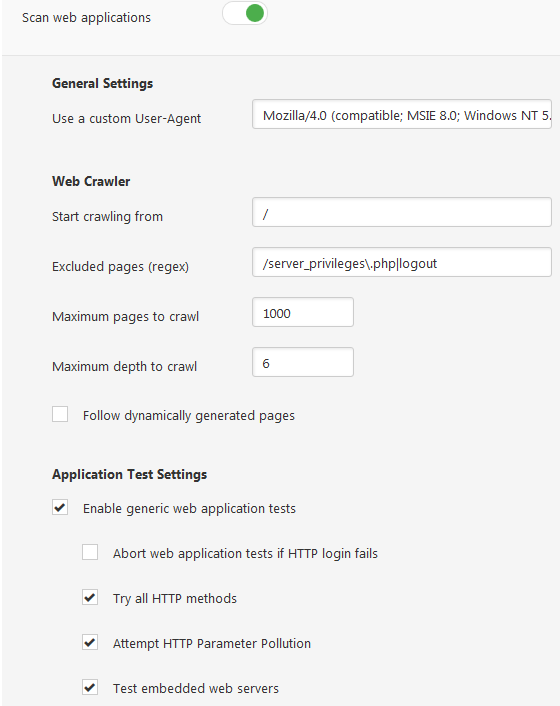
\includegraphics[width=\textwidth]{Nessus_9.png}
 \captionof{figure}{Advanced scan settings.}
\end{minipage}
$\;$ \\ \\
\noindent\begin{minipage}{\textwidth}
    \centering
    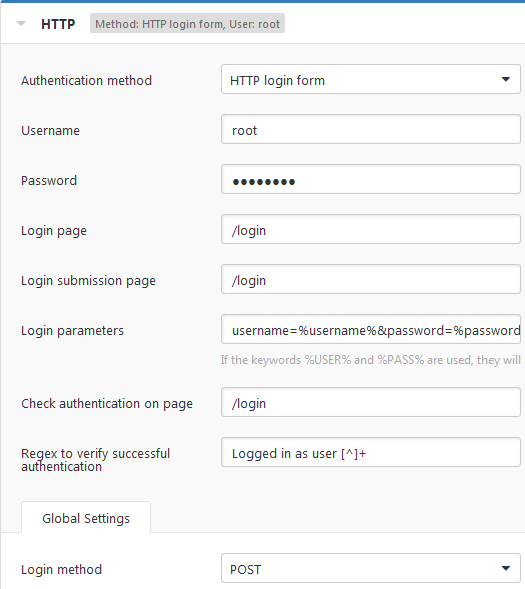
\includegraphics[width=\textwidth]{Nessus_10.png}
 \captionof{figure}{Advanced scan settings.}
\end{minipage}
$\;$ \\ \\
\noindent\begin{minipage}{\textwidth}
    \centering
    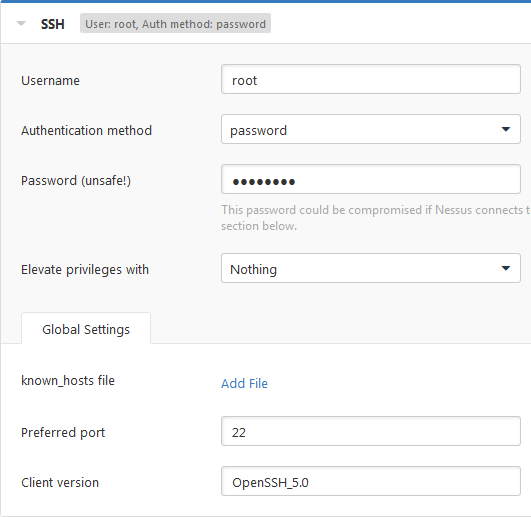
\includegraphics[width=\textwidth]{Nessus_11.png}
 \captionof{figure}{Advanced scan settings.}
\end{minipage}
$\;$ \\ \\
\noindent\begin{minipage}{\textwidth}
    \centering
    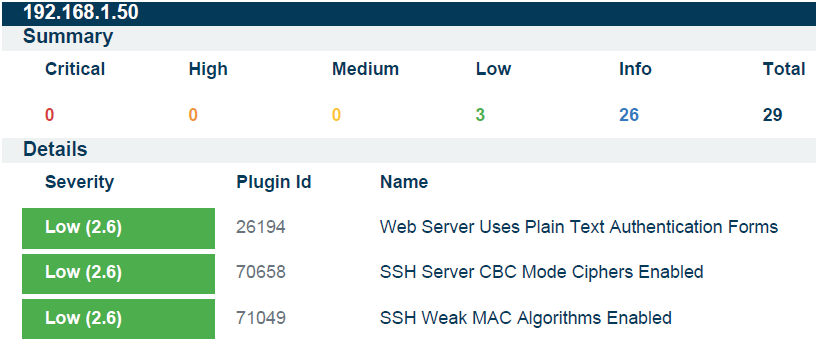
\includegraphics[width=\textwidth]{Nessus_12.png}
 \captionof{figure}{The three vulnerabilities.}
\end{minipage}
$\;$ \\ \\
So to summarize the advanced scan options and the web application scan options: 
\begin{itemize}
\item Scan TCP éand UDP ports 1-65565 using SYN scan + TCP, ARP, UDP and ICMP. Also OS detection and service detection was enabled.
\item The credentials were supplied, so netstat was used.
\item The web applications were crawled from the root.
\item Port enumerators (this enumerates ports via netstat, SNMP and WMI - reduces false positives) used are SSH, WMI and SNMP.
\item Web application scan using the Mozilla/4.0 starting from the root. All HTTP methods are tried and embedded web servers are also scanned.
\item To optimize functionality of the scan, a HTTP and SSH login sequence was created.
\end{itemize}

Local Port Enumerators: SSH (netstat), WMI, SNMP
Service discovery: probe all ports + known SSL ports

\section*{Conclusions}

Is the vSRX virtual firewall a secure device? Sure, as long as the web interface is not enabled. An analysis of the website performed by various web scanners reported that the website is susceptible to some attacks. \\
 When SSH or HTTP access is enabled (required actually to be able to manage the device remotely - although HTTP is not necessary required, one can perfectly manage the device from command line) the device becomes vulnerable. It is very easy to determine the running services, the OS version, webserver version, etc \ldots. A solution could be to login via RDP and ``locally'' manage the vSRX. \\
Good thing is that all the ports are closed by default as various scans reveil. However, some UDP ports are opened by default. \\
The vSRX is more or less resistant against a DOS. Only in one of three attempts the device did not respond anymore after the DOS had been performed. \\ \\
Is the vSRX virtual firewall a secure device? Sure, as long as the web interface and SSH are not enabled.

\section*{Planning}



\section*{Problems}



\section*{Issues}



\section*{Assistance}

\newpage

\section*{Appendix}

The complete scan report by Nessus is included as appendix.

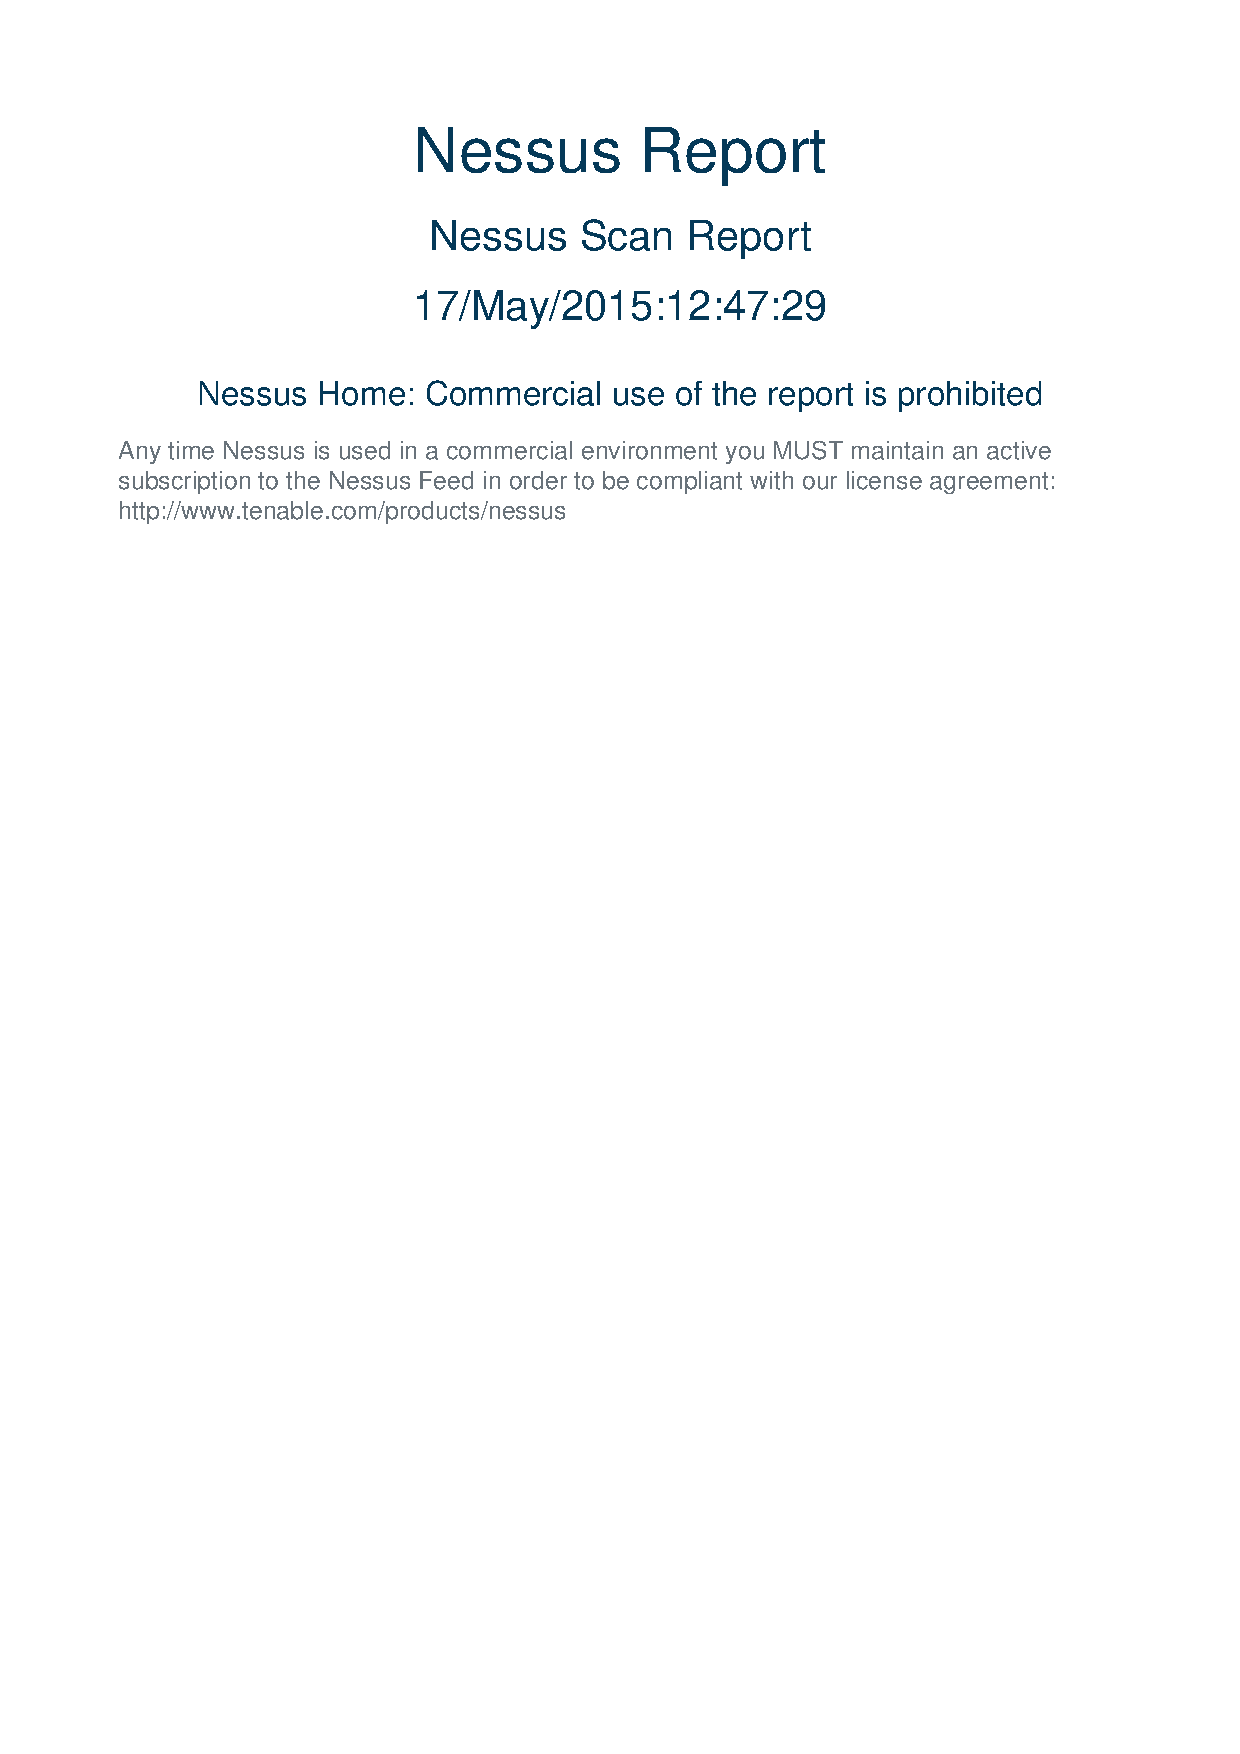
\includepdf[pages={1,2,4-34}]{Juniper_Advanced_Scan_Thorough.pdf}

\newpage

\bibliographystyle{apalike}
\bibliography{SITREP19}



\end{document}